\documentclass[10pt,a4paper]{article}
\usepackage[utf8]{inputenc}
\usepackage[english]{babel}
\usepackage{amsmath}
\usepackage{amsfonts}
\usepackage{amssymb}
\usepackage{graphicx}
\usepackage[left=2cm,right=2cm,top=2cm,bottom=2cm]{geometry}
\author{Marco Biroli}
\usepackage{physics}
\usepackage{stmaryrd}
\title{Master ENS ICFP - First Year 2020/2021\\
Relativistic Quantum Mechanics and Introduction to Quantum Field Theory\\
Mid Term Homework}

\begin{document}
\maketitle

\section[Exercise]{Some operator identities : 6 points}

\begin{enumerate}
\item We have that:
\[
e^A B e^{-A} = \sum_{n = 0}^{\infty} \frac{A^n}{n!} B \sum_{n = 0}^{+\infty} \frac{(-A)^n}{n!} = \sum_{n, m = 0}^{+\infty} \frac{A^n B (-A)^m}{n!m!} = \sum_{n, m = 0}^{+\infty} (-1)^m \frac{A^n B A^m}{n! m!} = \sum_{n = 0}^{+\infty} \frac{A^n}{n!} \sum_{m = 0}^{+\infty} (-1)^m \frac{BA^m}{m!}
\]
...

\item ...

\item We have that:
\[
[F, G^\dagger] = [\sum_j f_j a_j, \sum_j g_j^\star a_j^\dagger] = \sum_{j, k = 0}^{+\infty} f_j g_k^\star [a_j, a_k^\dagger] = \sum_{j, k = 0}^{+\infty} f_j g_k^\star \delta_{jk} = \sum_{j = 0}^{+\infty} f_j g_j^\star
\]
Furthermore we have that $[F, G^\dagger] \propto \text{Id}$ and therefore we trivially have that $[F, [F, G^\dagger]] = [G^\dagger, [F, G^\dagger]] = 0$. Now applying question 2 we have that:
\[
e^{G^\dagger} e^F = e^{-\frac{1}{2} \sum_{j} f_j g_j^\star } e^{G^\dagger + F} \Rightarrow  e^{\frac{1}{2} \sum_{j} f_j g_j^\star }e^F =  \underbrace{e^{\frac{1}{2} \sum_{j} f_j g_j^\star } e^{-\frac{1}{2} \sum_{j} f_j g_j^\star }}_{=e^A e^{-A}} e^{G^\dagger + F}
\]
Now from Question 1 we have that for any $A$ (trivially $[A, \text{Id}] = 0$) we get:
\[
e^A \text{Id} e^{-A} = \text{Id} + \sum_{n=1}^{+\infty} \frac{1}{n!} \cdot 0 = \text{Id}
\]
Hence the above formula simplifies to:
\[
e^{F + G^\dagger} = e^{\frac{1}{2}\sum_j f_jg_j^\star} e^{G^\dagger} e^F
\]

\item Similarly as before let $F = \int \dd^3 \vb{q} f(\vb{q}) a(\vb{q})$ and $G = \int \dd^3 \vb{q} h(\vb{q})^\dagger a(\vb{q})$. Then we have that:
\[
[F, G^\dagger] = [ \int \dd^3 \vb{q} f(\vb{q}) a(\vb{q}), \int \dd^3 \vb{q} h(\vb{q}) a^\dagger(\vb{q})] = \int \dd^3 \vb{q} f(\vb{q})h(\vb{q})[a(\vb{q}), a^\dagger(\vb{q})] = \int \dd^3 \vb{q} f(\vb{q}) h(\vb{q})
\]
A similar direct application of 2 gives the desired result.

\end{enumerate}

\section[Exercise]{An example of an asymptotic series}

We have that:
\[
f(g) = \frac{1}{\sqrt{\pi}} \int_{-\infty}^{+\infty} \dd x e^{-x^2 - g x^4} \mbox{~~hence~~} |f(g)| < \int_{-\infty}^{+\infty} \dd x | e^{-x^2 - g x^4}| = \int_{-\infty}^{+\infty} \dd x e^{-x^2 - x^4 \Re g} < \int_{-\infty}^{+\infty} \dd x e^{-x^4 \Re g}
\]
Hence as long as $\Re g > 0$ this is obviously well defined from the last term and if $\Re g = 0$ this is obviously well defined from the before last term.

\begin{enumerate}
\item This integral admits an exact solution given by:
\[
f(g) = \frac{e^{\frac{1}{8g}} K_{\frac{1}{4}}(\frac{1}{8g})}{2\sqrt{\pi g}} \delta_{\Re g > 0} + \delta_{\Re g = 0} \mbox{~~where~~} K_n(z) \mbox{~~is the modified Bessel function of the second kind.}
\]
The plot of the numerical values for $g \in [0.01, 1]$ is given in Figure \ref{integral:1}.
\begin{figure}
\centering
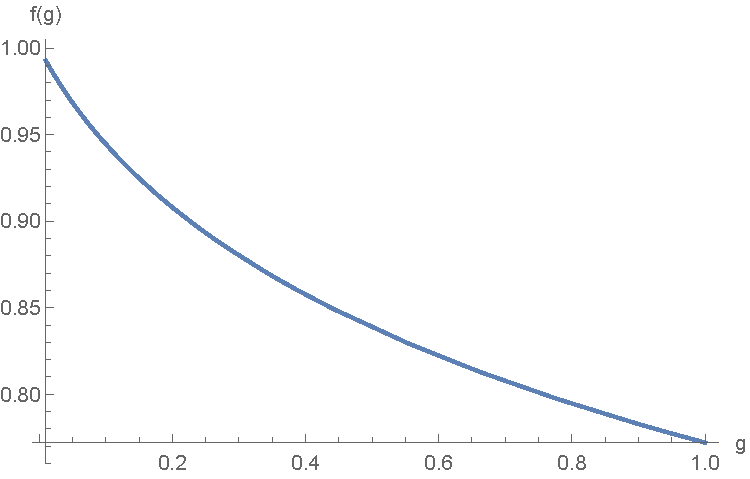
\includegraphics[width = 0.5\textwidth]{integral1}
\caption{Plot of the numerical values of $f(g)$ for $g \in [0.01, 1]$. }\label{integral:1}
\end{figure}
Then $f(g)$ decreases monotonically when $g > 0$ increases since:
\[
\dv{}{g} f(g) = \frac{1}{\sqrt{\pi}} \int_{-\infty}^{+\infty} \dd x (-x^4) e^{-x^2 - g x^4} = \frac{-1}{\sqrt{\pi}} \underbrace{\int_{-\infty}^{+\infty} x^4 e^{-x^2 - g x^4}}_{ > 0 \mbox{~~when~~} g \in \mathbb{R}^+} < 0
\]

\item We have that:
\[
e^{-g x^4} = \sum_{n = 0}^{+\infty} \frac{(-gx^4)^n}{n!}
\]
And plugging this in the expression of $f$ and inverting the sum and the integral gives:
\[
\frac{1}{\sqrt{\pi}} \sum_{n = 0}^{+\infty} \frac{(-g)^n}{n!} \int_{-\infty}^{+\infty} \dd x\,\, x^{4n} e^{-x^2}
\]
We notice the integral ressembles strongly the gamma function hence we change variables by taking $u = x^2$ ($\dd u = 2 \sqrt{u} \dd x$) and we get:
\[
2^{-1} \int_{-\infty}^{+\infty} \dd u u^{2n - \frac{1}{2}} e^{-u} = 2^{-1} \Gamma(2n + \frac{1}{2}) = 2^{-4n} \sqrt{\pi} \frac{\Gamma(4n)}{\Gamma(2n)} \mbox{~~from the Legendre duplication formula.}
\]
Hence plugging it back up top we obtain:
\[
\tilde{f}(g) = \sum_{n = 0}^{+\infty} \left( \frac{(-1)^n(4n)!}{n! 2^{4n} (2n)!} \right) g^n
\]
Notice that the terms $f_n$ are monotonically increasing in norm and diverge hence the sum does not converge absolutely and $R = 0$ and it also does not converge conditionally. The order of magnitude of the first few terms is ...

\item \begin{figure}
\centering
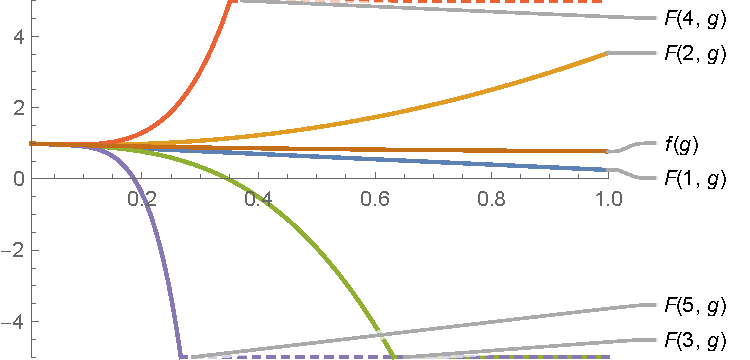
\includegraphics[width=0.44 \textwidth]{approx_series}
\hspace{0.1\textwidth}
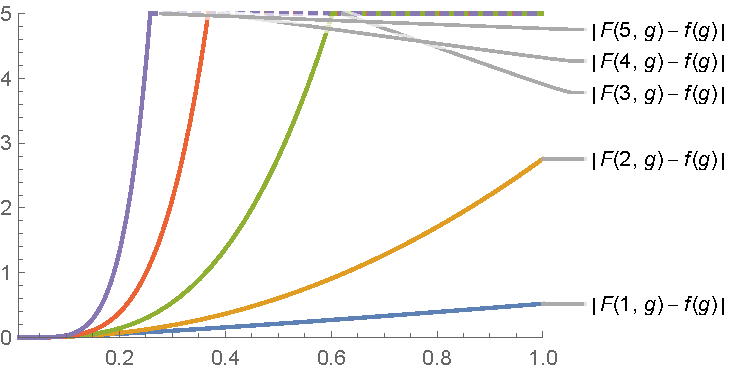
\includegraphics[width=0.44 \textwidth]{error_series}
\caption{Series approximations of $f(g)$ and their errors for $g \in [0.01, 1]$.}
\end{figure}

\end{enumerate}


\section{A relation between Dirac spinors}

\begin{enumerate}

\item We have that:
\[
...
\]

\item ...


\end{enumerate}


\section{Some traces of products of $\gamma$-matrices}

We have that:
\[
\tr \gamma_\mu \gamma_\nu = \tr {\gamma_\mu, \gamma_\nu} - \gamma_\nu \gamma_\mu = 2 \tr \eta_{\mu \nu} I_4 - \tr \gamma_\nu \gamma_\mu = 2 \tr \eta_{\mu \nu} I_4 - \tr \gamma_\mu \gamma_\nu
\]
Hence adding on both side we obtain the desired equality:
\[
\tr \gamma_\mu \gamma_\nu = \eta_{\mu \nu} \tr I_4 = 4 \eta_{\mu \nu}
\]
Similarly we have that:
\[
\tr \gamma_\mu \gamma_\nu \gamma_\rho \gamma_\sigma = ... 
\]

\section{Energy levels of a relativistic charged spin-0 particle in a harmonic electrostatic potential}

\begin{enumerate}


\item From these relation we have that:
\begin{align*}
X^2 \ket{n} &= \frac{1}{2 m \Omega} \left( a^2 + (a^\dagger)^2 + \{a, a^\dagger\} \right)\ket{n} \\
&= \frac{1}{2m \Omega} (\sqrt{n}\sqrt{n-1} \ket{n-2} + \sqrt{n+1}\sqrt{n+2} \ket{n+2} + (n+1)\ket{n} + n\ket{n})
\end{align*}
Hence we get that:
\[
\bra{n} X^4 \ket{n} = (\bra{n} X^2)(X^2 \ket{n}) = \frac{1}{(2 m \Omega)^2} (n^2 - n + n^2 + 3n + 2 + n + 1 + n) = \frac{2n^2 + 4n + 3}{(2m \Omega)^2}
\]

\item ...

\end{enumerate}

\section{The axial current}

\section{Supersymmetry}

\end{document}